\documentclass[12pt]{article}
%compile using XeLaTeX
\usepackage{diary_style}
\usepackage{subcaption}
\usepackage{graphicx}
\setlength{\footskip}{\paperheight
  -(0.75in+\voffset+\topmargin+\headheight+\headsep+\textheight)
  -0.75in}

\fontspec{Times New Roman}

\DeclareMathOperator{\di}{d\!}
\newcommand*\Eval[3]{\left.#1\right\rvert_{#2}^{#3}}

\begin{document}

%\doublespacing
\vspace{1.0 \baselineskip}

\begin{flushright}
	Alexander Caines\\
	MATH-310\\
	3-1-2021\\
\end{flushright}

\begin{center}
	\textbf{\underline{Midterm 1}}
\end{center}


%\vspace{0.5 \baselineskip}

\begin{enumerate}
	\item[1.] Given the results of the ANOVA, because the p value is less than 0.001,
		the intergroup differences are statistically significant.
		So, there is at least one area whose cotton candy levels are more dangerous.
		\begin{figure}[!h]
			\centering
			
\includegraphics[width=11cm]{p1.JPG}
		\end{figure}
	\item[2.] 
		\begin{enumerate}
			\item[(a)] The true average difference in translation between dominant 
				and nondominant arms for pitchers is 1.028 mm. 
			\item[(b)] The true average difference in translation between dominant 
				and nondominant arms for position players is 0.145 mm. 
			\item[(c)] I would agree as the sde calculated for pitchers was 0.959, 
				whereas the sde calcualted for position players was 0.367.
		\end{enumerate}
		\begin{figure}[!h]
			\centering
			\begin{subfigure}[b]{0.4\linewidth}
				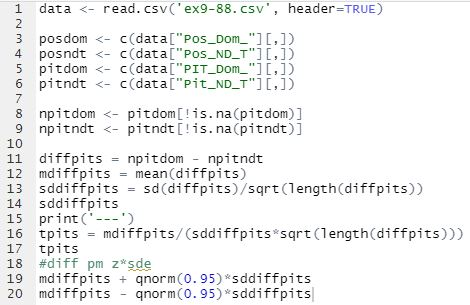
\includegraphics[width=7cm]{p2.JPG}
			\end{subfigure}
			\begin{subfigure}[b]{0.4\linewidth}
				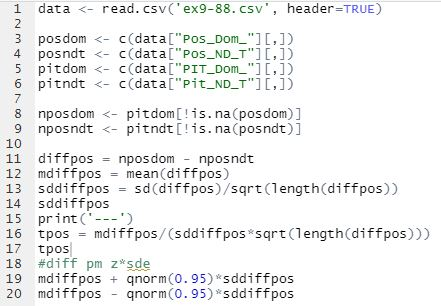
\includegraphics[width=7cm]{p2b.JPG}
			\end{subfigure}
		\end{figure}
\end{enumerate}
\newpage
\begin{enumerate}
	\item[3.] For this case, we would want to use a paired t-test, as 
		the diets were randomly assigned, each population was normally distributed, and their variances were similar.
		\begin{figure}[!h]
			\centering
			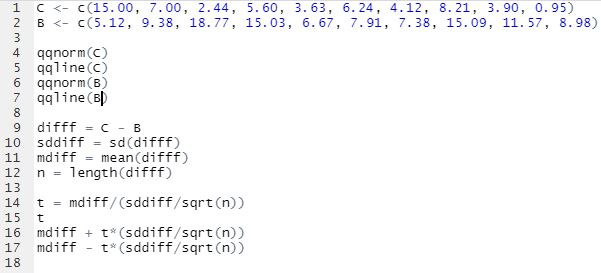
\includegraphics[width=11cm]{p3.JPG}
		\end{figure}
		\begin{figure}[!h]
			\centering
			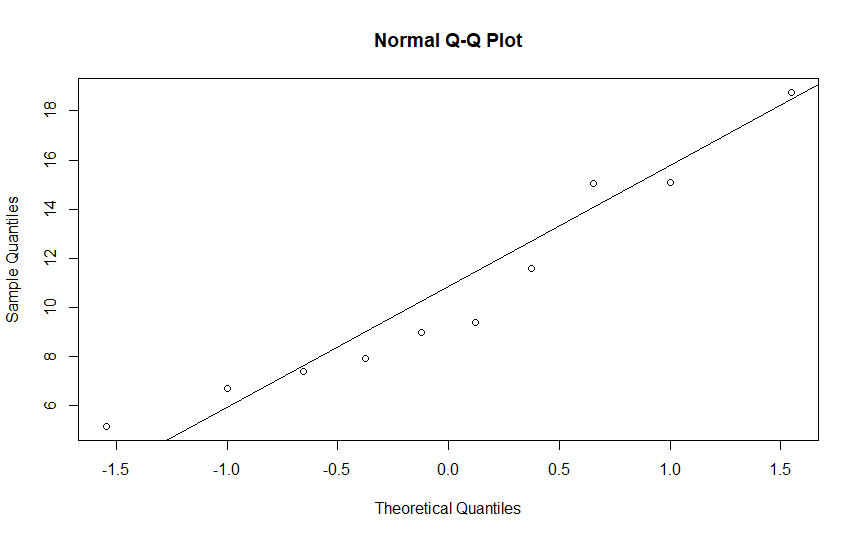
\includegraphics[width=11cm]{plotB.png}
			\caption{Proof of normality for population B.}
		\end{figure}
		\begin{figure}[!h]
			\centering
			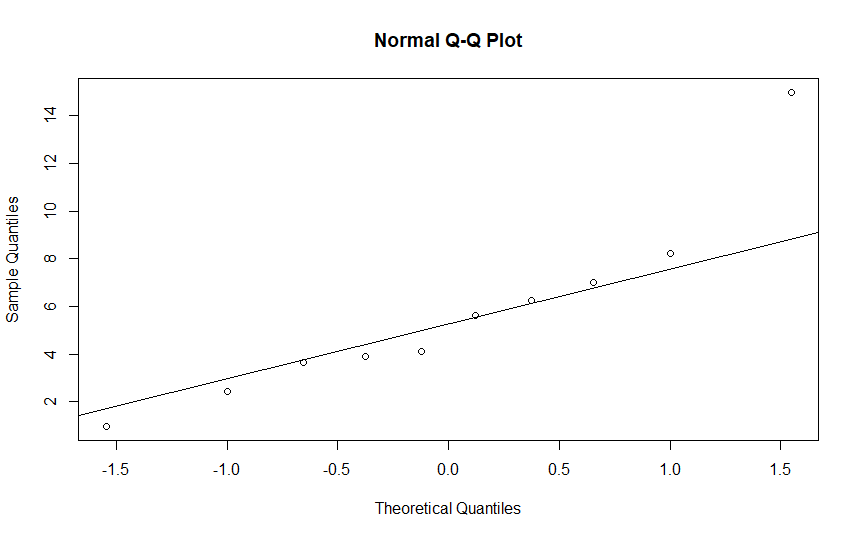
\includegraphics[width=10cm]{plotC.png}
			\caption{Proof of normality for population C.}
		\end{figure}
\end{enumerate}
\begin{enumerate}
	\item[4.] $\frac{\sigma^2_1}{\sigma^2_2} \cdot F_{1-\alpha/2, v_2, v_1} < \frac{\sigma^2_1}{\sigma^2_2} < \frac{\sigma^2_1}{\sigma^2_2} \cdot F_{\alpha/2, v_2, v_1}$
\end{enumerate}
\end{document}
